\documentclass[12pt,a4paper]{article}
\usepackage[utf8]{inputenc}
\usepackage[sfdefault]{roboto}
\usepackage[T1]{fontenc}
\usepackage{xcolor}
\usepackage{amsmath}
\usepackage{amsfonts}
\usepackage{amssymb}
\usepackage{ngerman}
\usepackage{amssymb}
\usepackage{microtype}
\usepackage{wrapfig}
\usepackage[left=2.5cm,right=2cm,top=2cm,bottom=2cm]{geometry}
\usepackage{graphicx}
\usepackage[style=authoryear]{biblatex}
\usepackage{setspace}
\onehalfspacing
\setlength{\parindent}{0pt}%Wenn Absatzabstand, dann Einzug unnötig

\begin{document}

\begin{titlepage}
\title{\vspace*{1cm} \huge{\textbf{SVM - Outdoor}} \\ \textbf{Webprojekt}\\
\textbf{Semester 2}\\
\vspace*{1cm}
\begin{figure}[htb]
\advance\leftskip-2cm

\includegraphics[scale=1.2]{Startseite.png}
\end{figure}
\vspace{2cm}}
\author{\textbf{1749577, 5223626, 5951911, 6310429, 7605326, 9080434}
\vspace*{5mm}\\
Webseite einsehbar unter: https://svm3.services.kostadinov.it/}
\date{\vspace{1cm} \textbf{15.06.2020}}

\end{titlepage}
\maketitle
\newpage
\tableofcontents
\newpage


\section{Rückblick}
\begin{wrapfigure}[16]{r}{5.5cm}
  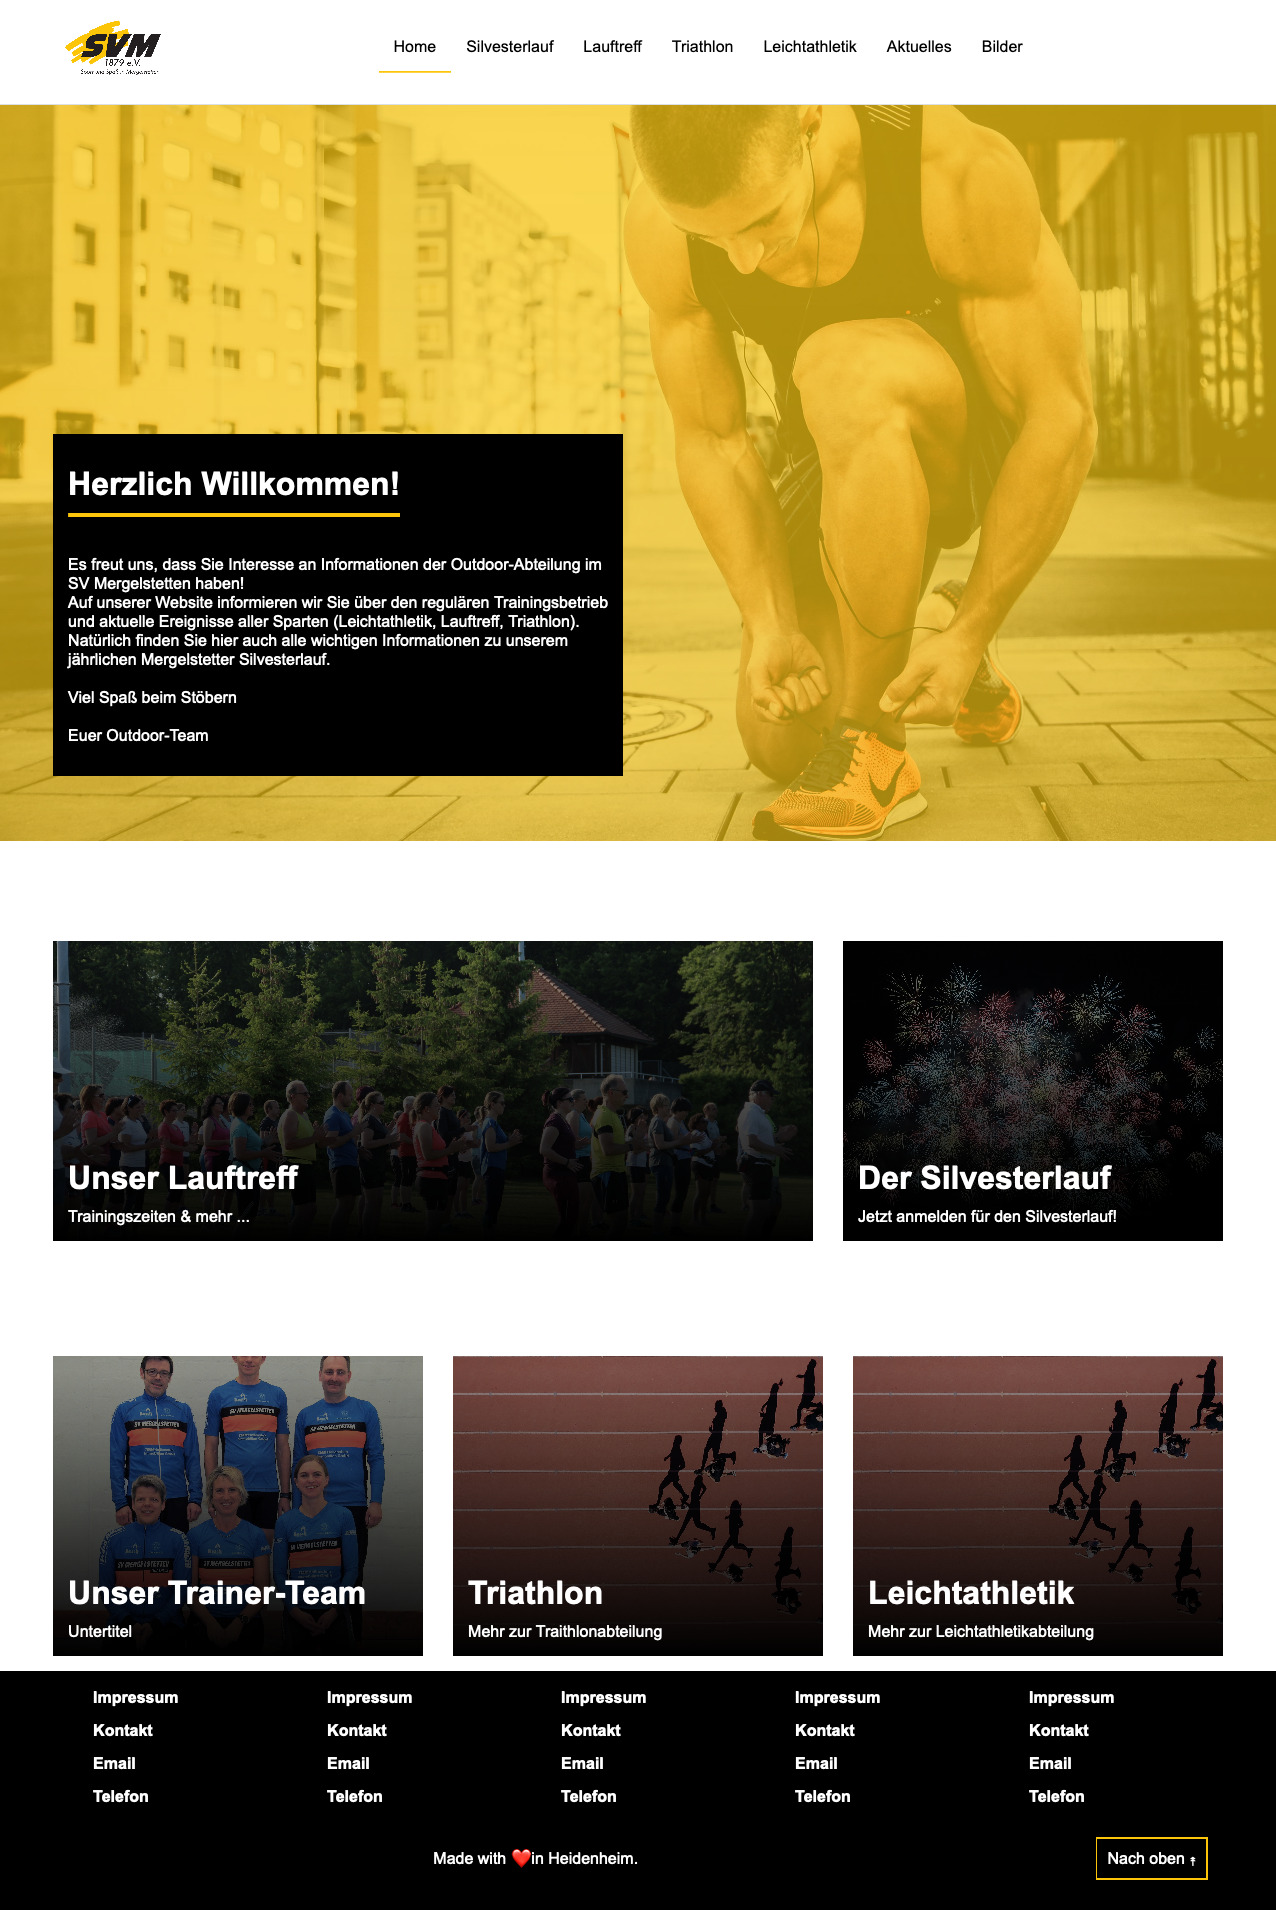
\includegraphics[width=5cm]{Home_Outdoor.jpg}
  \caption{Bisherige Desktop Ansicht}
  \label{img:Home_Outdoor_alt}
\end{wrapfigure}
Inhalt dieses gesamten Projekts ist die Erstellung einer Webseite für die Abteilung \glqq Outdoor\grqq \ des SV Mergestetten 1879 e.V.. \\
Hierbei sollen die Studierenden die Webentwicklung praktisch erlernen und gleichzeitig Aspekte des Projektmanagements kennenlernen und umsetzen.\\
Im ersten Semester musste jedes Team sich mit der Gestaltung einer statischen Webseite auseinander setzen. Die genauen Interpretationen des \glqq statischen Ansatzes\grqq \ unterschieden sich hierbei. Das Team hatte sich für folgende Definition entschieden: 
\begin{quote}
Bereitstellung von vorher erstellten Dateien auf einem Webserver.
\end{quote}
Für jeden Betrachter der Webseite waren also alle Inhalte stehts gleich und Änderungen mussten direkt an den auf dem Webserver bereitgestellten Dateien durchgeführt werden.\\\par\smallskip
In Abbildung \ref{img:Home_Outdoor_alt} ist der bisherige Stand der statischen Webseite in der Desktop Ansicht zu sehen. Im aktuellen Semester, also beim Übergang von statisch zu dynamisch, sollten Designelemente wie der \glqq Hero\grqq, also das jeweilige Titelbild jeder Unterseite und der\glqq Footer\grqq, die Fußzeile jeder Seite, erhalten bleiben.\\
Auch die mobile Ansicht, beziehungsweise das responsive Design, war Kernbestandteil des vergangenen ersten Semesters, was natürlich beibehalten, ausgebaut und verbessert werden sollte.



\section{Problemstellung}
Wie bereits beschrieben war es Ziel dieses Teils des Projekts im zweiten Theorie-Semester die statische Webseite in eine dynamische zu überführen. Auch der Begriff \glqq dynamisch\grqq \ im gegeben Kontext musste erst einmal genau beleuchtet und definiert werden:
\begin{quote}
Seiteninhalte und -daten werden dynamisch beim Aufruf der Seite geladen und zusammengesetzt.
\end{quote}
Den Teams war es freigestellt, ob sie ihren bisherigen Stand der Seite aus- und umbauen oder direkt auf das vom Hauptverein genutzte Content Management System, kurz \glqq CMS\grqq, umsteigen. Beide Varianten haben spezifische Vor- und Nachteile.\\
Der Umbau der bestehenden Seite von statisch auf dynamisch ermöglicht den Teammitgliedern einen tieferen Einblick in die Webprogrammierung mit PHP, lässt aber gleichzeitig einen höheren Arbeitsaufwand für die folgenden Semester.\\
Die Verwendung des CMS Joomla\footnote{\label{foot:Joomla} https://www.joomla.de/} bietet dem Team hingegen einen direkten Einblick in solche Content Management Systeme, die Unternehmen als \glqq Sammlung von Werkzeugen und Methoden zur Unterstützung von Web Content Management\grqq\footnote{\label{foot:CMS} Spörrer S. (2009): Content Management Systeme, S. 26} dienen. Die Einrichtung eines solchen CMS erfordert jedoch auch einen hohen Initialaufwand, sodass die Wahl einer der beiden Varianten gut überlegt sein muss.



\section{Lösungsansatz}
Aus den genannten Optionen entschied sich das Team dafür direkt das CMS Joomla zu verwenden. Ziel sollte es sein, die bestehende statische Seite\footnote{\label{foot:Alte_Seite} http://www.1.projekt.dhbw-heidenheim.de/} mit ihrem grundlegenden Design und den wichtigsten Elementen zu übernehmen und zu verbessern.\\
Außerdem sollen weitere Funktionalitäten hinzugefügt werden. Hierzu zählen:
\begin{itemize}
\item ein Login zu einem \textbf{internen Bereich}
\item eine \glqq \textbf{404 - Page not found}\grqq \ Seite
\item eine \textbf{einfache, intuitive Oberfläche} zum Ändern von Seiteninhalten
\item eine Suche
\item ein Favicon
\item die Einbindung von \textbf{interaktivem} Kartenmaterial
\item ein \textbf{ausklappbares Menü}
\end{itemize}
Jede dieser und weitere Umsetzungen werden später im Kapitel \ref{sec:Umsetzung} thematisiert, ausgeführt und erklärt.\\
Ein zusätzliches Ziel war es, geeignte Tools zu finden, die in Kapitel \ref{subsec:Tools} beschrieben werden und die die Erweiterbarkeit der Seite nicht begrenzen, um auch im dritten und vierten Teil der Projektarbeit weitere Entwicklungen an der Seite zu ermöglichen.


\newpage
\section{Projektmanagement}
Wie im vergangenen Semester wurde auch in diesem Semester der \glqq hybride Managementansatz\grqq \ gewählt. 
\begin{quote}
Unter hybridem Projektmanagement versteht man die Kombination aus dem klassischen und agilen Projektmanagement. Das Projekt wird hierbei in klassische Phasen gegliedert, in denen innerhalb agile Ansätze verfolgt werden.\footnote{\label{foot:hybrid} Vgl. Marquart R., Pifczyk A. (2019): Wissens Management}
\end{quote}
Um sowohl die Phasen selbst, als auch die einzelnen Aufgaben innerhalb einer Phase besser als im letzten Semester beobachten und durchführen zu können, sollte in diesem Semester ein Projektmanagement-Tool eingesetzt werden.\\
In der Vorlesung \glqq Systemanalyse und -entwurf\grqq \ wurden verschiedene Anbieter und Tools vorgestellt. Schlussendlich wurde Jira\footnote{\label{foot:Jira} https://www.atlassian.com/de/software/jira} in Verbindung mit einem Kanban Board\footnote{\label{foot:kanban} https://www.atlassian.com/de/agile/kanban/boards} gewählt.\\


\subsection{Kanban Board}
\begin{figure}[htbp]
  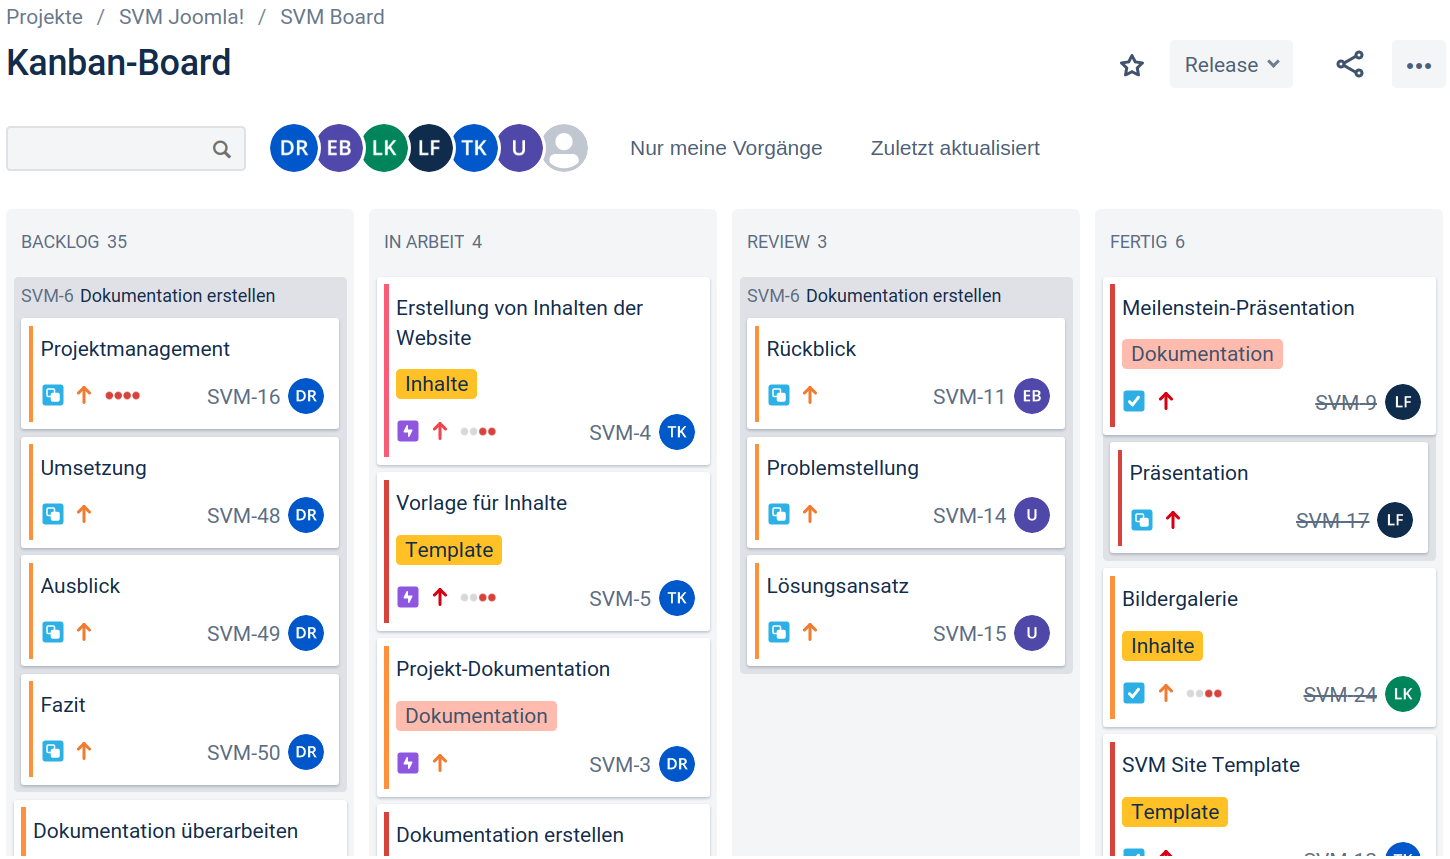
\includegraphics[width=\textwidth]{KanbanSVM.png}
  \caption{Kanban Board}
  \label{img:KanbanBoard}
\end{figure}
Ein solches \textbf{Kanban Board} wird üblicherweise in drei oder mehr Spalten unterteilt, welche einen bestimmten Zustand der darin befindlichen Elemente definieren. Im Fall des vorliegenden Projekts entschied man sich, wie in Abbildung \ref{img:KanbanBoard} zu sehen, für vier solcher Spalten:
\paragraph{Backlog} Im \textit{Backlog} werden sämtliche Elemente geführt, die noch bearbeitet werden müssen.
\paragraph{In Arbeit} Hier stehen alle Elemente die aktuell bearbeitet werden.
\paragraph{Review} In dieser Spalte ist alles zu finden, was durch andere Teammitglieder abgenommen werden muss.
\paragraph{Fertig} Alle bearbeiteten und überprüften Elemente werden hierher verschoben und damit als erledigt verbucht.


\subsection{Aufgabenkategorisierung}
Um Aufgaben des Projekts gliedern zu können wurden \textbf{Epics, Tasks und Sub-Tasks} erstellt.
Ein Epic, wie es beispielhaft in Abbildung \ref{img:Epic} zu sehen ist, enthält ein oder mehrere Tasks. Unter einen Task fallen wiederum ein oder mehrere Sub-Tasks. Die Epics stellen also die oberste Schicht der Gliederung dar:
\paragraph{Template} Dieses \textit{Epic} umfasst sämtliche Tasks zur Erstellung des Joomla-Templates und war zentral zum Beginn der tatsächlichen Arbeit an der Webseite.
\paragraph{Inhalte} Dem Wort direkt zu entnehmen, befasst sich dieses \textit{Epic}, welches auch in Abbildung \ref{img:Epic} mit seinen Tasks zu sehen ist, mit der Implementierung der gestellten Inhalte.

\paragraph{Testen} 
\begin{wrapfigure}[10]{r}{9.5cm}
  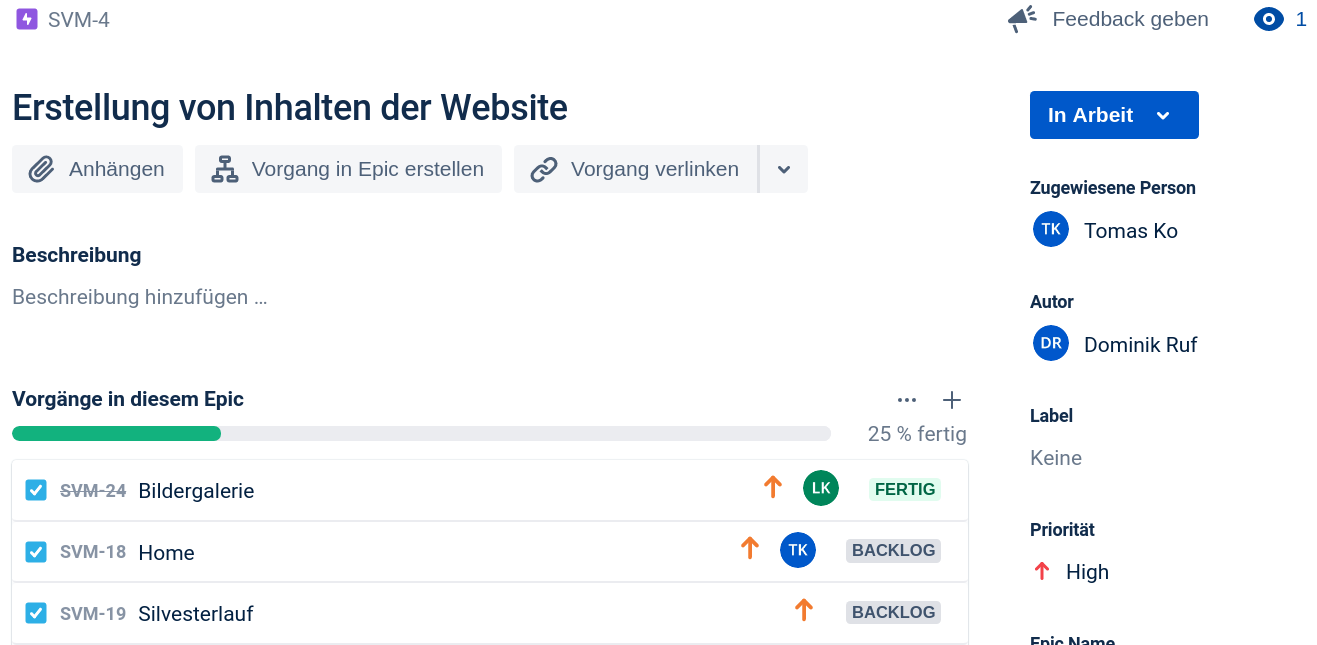
\includegraphics[width=9cm]{Epic.png}
  \caption{Epic}
  \label{img:Epic}
\end{wrapfigure}
Zentraler Punkt eines Projekts ist vor dem Rollout immer das Testen, weshalb hierfür ein extra \textit{Epic} mit der höchsten Priorität angelegt wurde.
\paragraph{Dokumentation} In diesem \textit{Epic} werden alle dokumentarischen Aufgaben, wie Präsentationen oder die Erstellung dieser Projektdokumentation, zusammengefasst.\\
\par\smallskip
Jedes dieser Epics umfasst, wie bereits oben beschrieben, mehrere Tasks und Sub-Tasks. Diese wurden vom Teamleiter nach Wissensstand und verfügbarer Zeit in der jeweiligen klassischen Phase des hybriden Managements zugeordnet. War in der laufenden Phase noch Zeit übrig, so konnten sich die Teammitgleider selbstständig weitere Aufgaben aus dem Backlog zuweisen.\\
So waren sämtliche Aufgaben immer klar verteilt und es konnte nicht passieren, dass einzelne vergessen oder Aufgaben mit hoher Priorität zu spät durchgeführt werden.


\subsection{Einfluss von COVID-19 auf das Projekt}
Natürlich hatte auch COVID-19 und die damit verbundenen Kontaktverbote einen sehr großen Einfluss auf das Projektmanagement und das Projekt selbst, der im folgenden kurz thematisiert werden soll.\\
Im vergangen ersten Semester wurden sämtliche Tätigkeiten, die Programmieraufwand oder administrative Tätigkeiten am Server oder der Seite selbst erforderten, stets bei einem Treffen durchgeführt. Dies ermöglichte jedem Teammitglied einen optimalen Einblick in alle Bereiche des statischen Webdesigns. Im aktuellen Semester war es notwendig hier andere Wege zu finden.
Die größte Umstellung war hierbei die Verwendung des oben beschriebenen Projektmanagement-Tools. Mit diesem war es möglich einzelne Aufgaben den Teammitgliedern direkt zuzuordnen und als Team den aktuellen Stand des Projekts stets genau analysieren zu können. Außerdem fanden Tools wie Microsoft Teams\footnote{\label{foot:Teams} https://www.microsoft.com/de-de/microsoft-365/microsoft-teams/group-chat-software} und Skype\footnote{\label{foot:Skype} https://www.skype.com/de/} Anwendung, um trotz der Umstände wieder Teamtätigkeiten durchführen zu können. Ein Großteil der \glqq Reviews\grqq \ fand während solcher Treffen statt, damit sämtliche Fortschritte von jedem Teammitglied gesehen, verstanden und abgesegnet werden konnten.





\section{Umsetzung}\label{sec:Umsetzung}
In diesem Kapitel wird die Umsetzung neuer, wichtiger Features und Elemente der Webseite beschrieben und erklärt. 


\subsection{Tools}\label{subsec:Tools}
\begin{wrapfigure}[10]{r}{7.cm}
  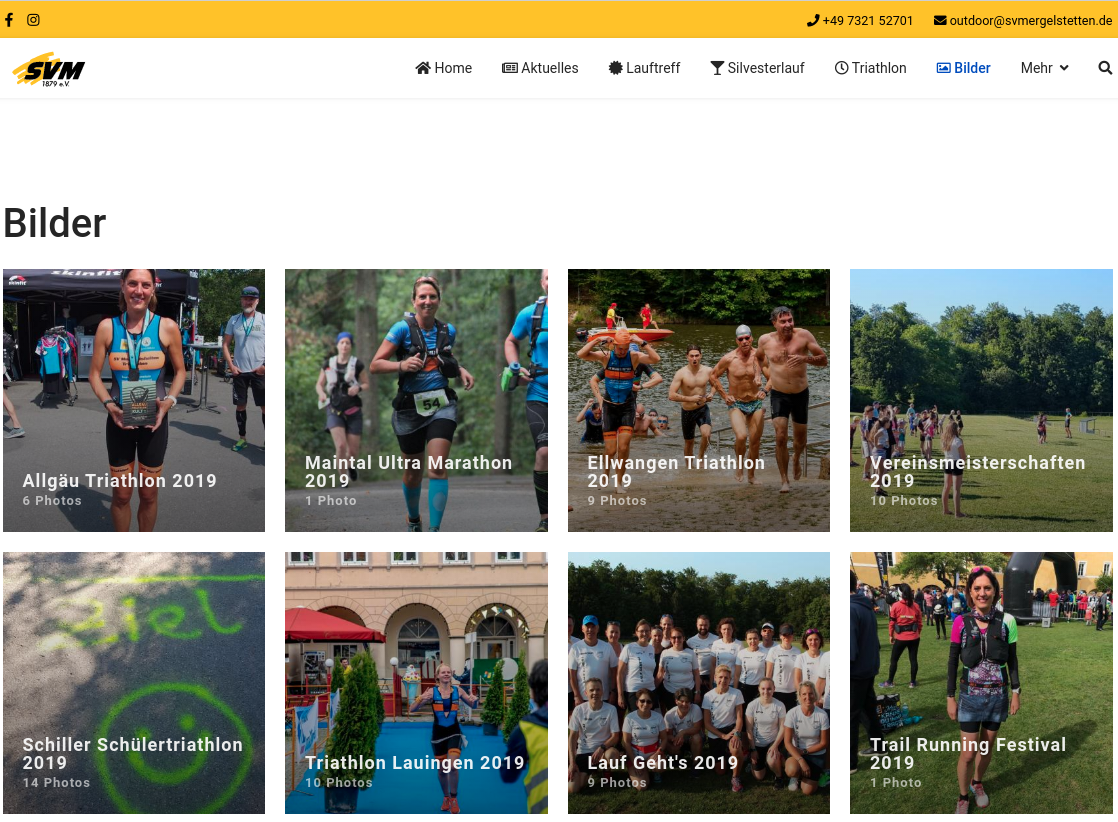
\includegraphics[width=6.5cm]{Bildergallerie.png}
  \caption{Bildergallerie}
  \label{img:Bildergallerie}
\end{wrapfigure}
Oberste Anforderung an das Projekt war es, eine einfache Änderbarkeit für Administratoren der Seite ohne weitreichende Programmierkentnisse zu erreichen. Um dies zu realisieren, wurde die Erweiterung \glqq SP Page Builder\grqq \footnote{\label{foot:SPPageBuilder} https://extensions.joomla.org/extension/sp-page-builder/} zu Joomla hinzugefügt. Diese Extension ermöglicht es sehr einfach Seiten per \glqq Drag \& Drop\grqq \ zu erstellen und abzuändern. \\
Zudem können eigene Desings mittels eigenem CSS erstellt werden. Im vorliegenden Fall wurden so beispielsweise die SVM Farben für die Seite festgelegt.\\
Damit auch Bilder von Veranstaltungen und Ähnlichem optisch ansprechend präsentiert werden können, wurde die Erweiterung \glqq SP Page Gallery\grqq \ hinzugefügt. Durch diese werden die einzelnen Gallerien und Bilder, wie in Abbildung \ref{img:Bildergallerie} zu sehen, als Mosaik angeordnet und können durch Anklicken in einer \glqq Pop-Up Gallerie\grqq \ geöffnet werden.


\subsection{Favicon}

Ein \textbf{Favicon} ist ein kleines grafisches Element, das verwendet wird, um einen gewissen Wiedererkennungswert bei Webseiten zu erreichen.
Bei der vorliegenden Webseite wurde sich für das SVM-Logo auf weißem Grund entschieden. Das Favicon erscheint sowohl am linken Rand des entsprechenden Tabs, als auch als Icon in der Lesezeichenleiste, wenn die Seite dort abgespeichert wird.


\subsection{404 Page}
\begin{wrapfigure}[8]{r}{4.5cm}
  
\includegraphics[width=4.5cm]{404.png}
  \caption{404 Page}
  \label{img:404}
\end{wrapfigure}
Hatten sich Besucher der Seite des ersten Projektteils sich bei der Webadresse vertippt oder zeigte ein Link auf eine beschädigte Adresse, so erhielt er stets die Meldung \glqq Cannot GET ...\grqq \ und musste eine neue Adresse eingeben oder zurück zur letzten besuchten Seite navigieren.\\
Mit der neuen, dynamischen Ausarbeitung werden die Besucher bei einem solchen Fehler auf die \glqq 404 - Page not found\grqq \ Seite, zu sehen in Abbildung \ref{img:404}, weitergeleitet und haben dort die Möglichkeit sich direkt zur Startseite zurücknavigieren zu lassen.

\subsection{Kontakte}
Ein zentraler Punkt des Webauftritts einer Sportabteilung ist immer auch die Möglichkeit den passenden Ansprechpartner zu finden. Um den Besuchern der Seite dies zu vereinfachen, wurde eine Kontaktübersicht erstellt, in der die einzelnen Kontaktpersonen mit ihrer Position aufgeführt sind. Wurde die richtige Kontaktperson gefunden, so kann durch Klicken des gleichnamigen Links die Kontaktseite aufgerufen werden. Dort findet man generelle Kontaktinformationen, die auch zum Download als \glqq vCard\grqq \ zur Verfügung stehen. Des weiteren besteht die Möglichkeit mit Hilfe des neu eingeführten Kontaktfomulars den Ansprechpartner direkt zu kontaktieren.

\newpage
\subsection{Menü und Suche}
\begin{wrapfigure}[14]{r}{7.5cm}
  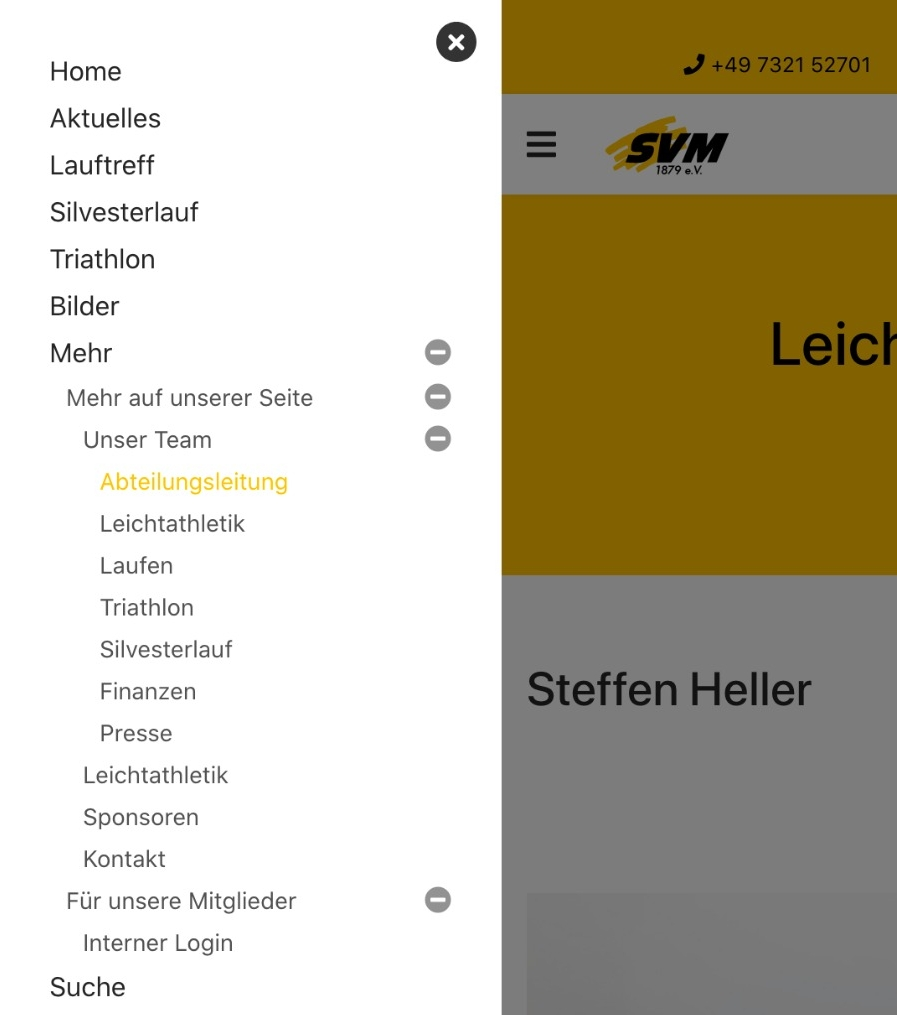
\includegraphics[width=7cm]{MenueMobile.jpeg}
  \caption{Mobile Menü}
  \label{img:MenueMobile}
\end{wrapfigure}
In der neuen, dynamischen Ausarbeitung der Webseite wurde auch das Menü überarbeitet. Unter \glqq Mehr\grqq \ ist es nun möglich weitere Menüpunkte aufzuklappen. Dies verhindert ein Überladen des Menüs und ermöglicht gleichzeigt mehr Inhalte direkt zu erreichen.\\
Auch das Menü im Mobilen Browser, wie es in Abbildung \ref{img:MenueMobile} zu sehen ist, wurde in diesem Zuge umgearbeitet und bietet den Besuchern sämtliche Funktionalitäten der Desktop Version.\\
Als neues Feature wurde der Menüleiste auch eine Suche hinzugefügt, die es für die Besucher ebenfalls möglich macht Gesuchtes gezielt zu finden.

\subsection{Arktikel}
Artikel über Veranstaltungen werden als \glqq News-Artikel\grqq \ eingebunden. Sie sind damit an verschiedenen Stellen, wie beispielsweise auch im Footer, zu verwenden. Dies lässt sich gerade in späteren Stadien der Seite und im live-Betrieb optimal nutzen, um die Besucher der Seite auf neue Inhalte aufmerksam zu machen.

\subsection{Verschlüsselung}
\begin{wrapfigure}[12]{r}{6.5cm}
  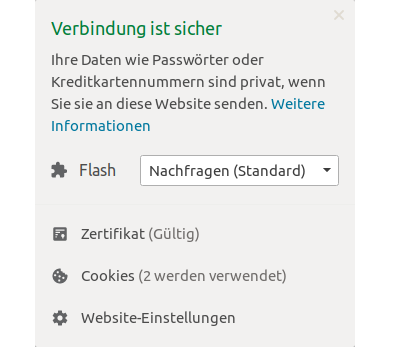
\includegraphics[width=6.0cm]{https.png}
  \caption{Website-Infomationen}
  \label{img:https}
\end{wrapfigure}
Bei der  Webseite aus dem letzten Semester erhielt man die Anzeige \glqq Die Verbindung zu dieser Webseite ist nicht sicher\grqq. Dies resultierte aus der Verwendung des http-Protokolls zur Übertragung von Daten zwischen Server und Client. Diese Übertragung war jedoch nicht abhörsicher und so hätten theoretisch Daten wie Passwörter und Kreditkartennummern gestohlen werden können.\\
Die neue Webseite verwendet nun das \textbf{Hypertext} \textbf{Transfer} \textbf{Protocol} \textbf{Secure}, kurz https, mit dem eine abhörsichere Datenübertragung gewährleistet ist.

\subsection{Interner Bereich}
Mitgliedern und Administratoren ist es je nach Einstellung möglich, sich über den Internen Login anzumelden und Inhalte der Seite  einzusehen, zu verändern und hinzuzufügen.\\
Desweiteren kann man sich dort auch registrieren und Informationen an seine registrierte Mail-Adresse senden lassen, sollte man sein Passwort oder seinen Benutzernamen vergessen haben. 


\section{Datenschutz}
\begin{wrapfigure}[14]{r}{5.5cm}
  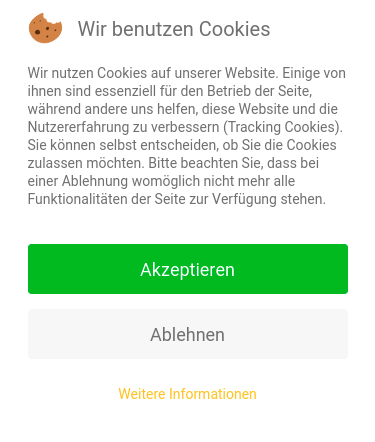
\includegraphics[width=5cm]{Cookies.png}
  \caption{Cookie Abfrage}
  \label{img:Cookie}
\end{wrapfigure}
Nach der Allgemeinen Datenschutz-Grundverordnung der EU ist jede Webseite dazu verpflichtet, allen Benutzern der Seite aus Europa die Kontrolle über die Aktivierung der Cookies und Tracker zu ermöglichen.\\
Dies wurde durch die Cookie-Zustimmungsabfrage beim ersten Besuch der Webseite gewährleistet. Besucher können, wie in Abbildung \ref{img:Cookie} zu sehen, die Verwendung von Cookies aktzeptieren, ablehnen oder weitere Informationen dazu erhalten.\\
Sollte die Verwendung von Cookies abgeleht werden, so werden extern gehostete Bilder, Kartenausschnitte und Ähnliches nicht mehr angezeigt.\\
In Abbildung \ref{img:CookiesAbgelehnt} ist das Resultat dieser Ablehnung sehr gut zu sehen.\\
\begin{figure}[htbp]
  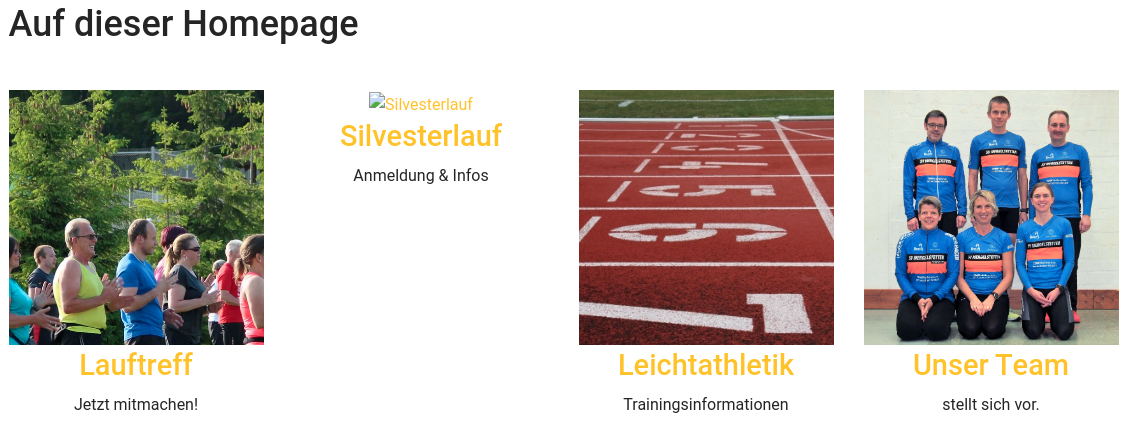
\includegraphics[width=\textwidth]{CookiesAbgelehnt.png}
  \caption{Startseite mit abgelehnten Cookies}
  \label{img:CookiesAbgelehnt}
\end{figure}



\section{Ausblick}
Natürlich konnte das Team im zweiten Abschnitt noch nicht alle gewünschten Features einbauen.
Dies lässt aber auch noch Entwicklungsmöglichkeiten für die folgenden zwei Projektabschnitte im dritten und vierten Semester.\\
Der \glqq SP Page Builder\grqq \ aus Kapitel \ref{subsec:Tools} bietet dem Anwender in der Pro-Variante eine Vielzahl weiterer Addons zur Gestaltung von Seiten der Webseite.\\
Ein großer Punkt, dem das Team noch viel Aufmerksamkeit schenken wird, ist die Kontakte-Seite.
\begin{wrapfigure}[9]{r}{6.5cm}
  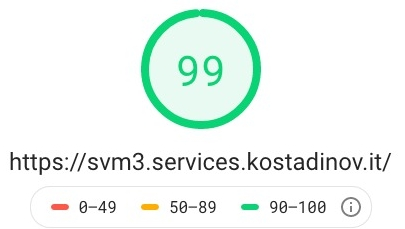
\includegraphics[width=6cm]{PageSpeedInsightsNeu.jpeg}
  \caption{PageSpeed Analyse}
  \label{img:PageSpeed}
\end{wrapfigure}
Diese Seite wird direkt aus den angelegten Kontakten generiert und unterliegt damit Standardeinstellungen von Joomla und dem SP Page Builder. Das Team ist mit der Gestaltung dieser Seite noch nicht zufrieden, konnte aber bisher noch keine Aufarbeitung dieser vornehmen.
Noch dazu erreicht die Seite leider bei PageSpeed Insights\footnote{\label{foot:PageSpeed} https://developers.google.com/speed/pagespeed/insights/} noch nicht konstant Bestwerte wie im letzten Semester. Auch hier möchte das Team weiter optimieren, um sowohl in der Dektop, als auch in der Mobilen Anaylse wieder eine sehr gute Bewertung zu erhalten.


\section{Fazit}
Abschließend lässt sich über das Projekt im zweiten Semester sagen, dass die Überführung der statischen Webseite in eine dynamische erfolgreich umgesetzt wurde. Die größten Schwierigkeiten ergaben sich für das Team aus den fehlenden Möglichkeiten von persönlichen Treffen, da der Wissensstand der einzelnen Teammitgliedern immer noch stark voneinander abweicht. \\
Dieser Unterschied konnte jedoch durch die Verwendung des Projektmanagement-Tools Jira und des Kanban-Boards optimal genutzt werden. So erhielten versierte Programmierer des Teams die Verantwortung für die Umsetzung des Progammieraufwands der Webseite. Programmier-Neulinge wurden so mit der Zuteilung von einfacheren Sub-Tasks herangeführt und bekamen in den Reviews stets einen hervorragenden Überblick über alle getätigten Schritte der Fortgeschrittenen.\\
Gleichzeitig waren die kreativ veranlagten Teammitgliedern verantwortlich für die unter dem Epic \glqq Dokumentation\grqq \ geführten Tasks. Auch hier wurden die nicht so versierten mit in die Erstellung der Dokumente und Präsentationen einbezogen, um  jedem Teammitglied Potential zur persönlichen Entwicklung zu bieten.
\begin{figure}[htbp]
  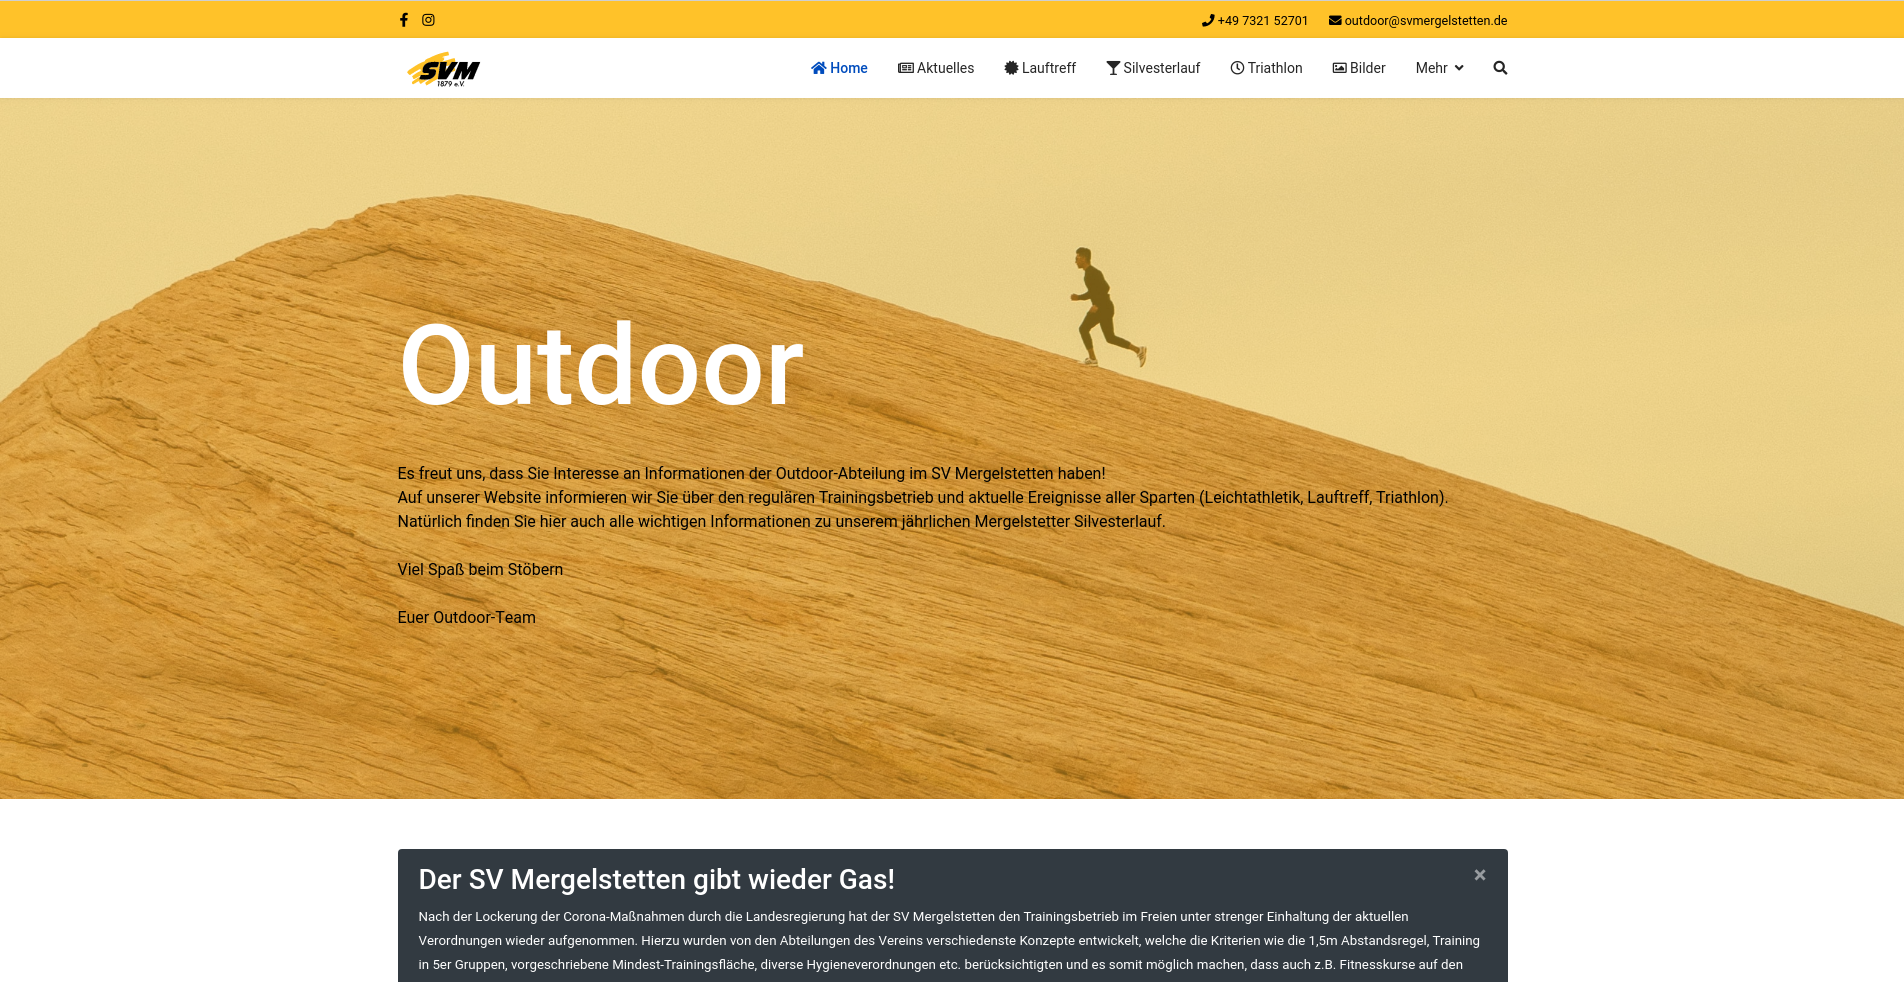
\includegraphics[width=\textwidth]{Endscreen.png}
  \caption{Aktuelle Startseite}
  \label{img:Startseite}
\end{figure}
\newpage
Im Allgemeinen ist sich das Team nun auch bewusst, den Aspekt des Projektmanagements im letzten Semester nicht optimal umgesetzt zu haben. Defizite in diesem Bereich konnten im laufenden Semester durch Reflexion abgebaut werden.\\
Das Team freut sich bereits jetzt auf die die Fortführung und die anstehenden Erweiterunge im dritten und vierten Semester.
\end{document}

